
\chapter*{Chapter 4}
\markboth{Sprint 2 : Network Testing \& Reports generation}{Sprint 2 : "Network Testing \& Reports generation} %pour afficher l'entete
 \addcontentsline{toc}{chapter}{4 Sprint 2 : Network Testing \& Reports generation}


\setcounter{chapter}{4}
\setcounter{section}{0}
\setcounter{table}{0} 
\setcounter{figure}{0} 


\etocsettocstyle{\subsection*{Plan}}{}
\vspace{0.25cm}

\setcounter{tocdepth}{1}
\headrule{
\vspace{0.5cm}

\begin{center}
    \textsc{\textbf {\Huge Sprint 2 : Network Testing \& Reports generation}} 
\end{center}
}
\headrule


\localtableofcontents
\newpage

\section*{Introduction}
After completing the first sprint and build the application's skeleton that we presented in the previous chapter, it's time to to go further and realize the rest of the functionalities .   
In this chapter, we will tackle the second sprint of our project which focuses on the "Network Testing \& Reports generation" .
We will cover its analysis, modeling, and realization.

\section{Sprint 2 Backlog}

The sprint backlog is a detailed list of tasks and user stories selected for completion within the current sprint, guiding the development team's work towards achieving the sprint goal. It serves as a dynamic, prioritized plan that evolves as the team progresses and new information emerges.
The table below describes the backlog of the second sprint :



\begin{table}[H]
    % \centering
    \renewcommand{\arraystretch}{1.2}
    \setlength{\belowcaptionskip}{0.25cm}
 
   \begin{tabular}{|p{0.05\textwidth}|p{0.2\textwidth}|p{0.34\textwidth}|p{0.34\textwidth}|}
   \hline
   \textbf{ID}  &  \textbf{User Story } & \textbf{Description} & \textbf{Task} \\ \hline


   
   \begin{center}
       \textbf{1}
   \end{center} & \begin{center}
       As a user, I want to test my network
   \end{center} &
   The user can perform a  network test and have results on network download and upload speed and latency, also he can  save the test result and give his evaluation.
   & 

       \begin{itemize}[left=0pt, label={\textbf{\Huge .}}]
       % \renewcommand\labelitemi{\textbf{\Huge .}}
            \item Develop the backend logic for testing the network
            \item Develop the user interface for  launching a test
            \item Develop the user interface for  saving result
            \item Develop the backend for managing  saved results
        \end{itemize} \\ \hline


   \begin{center}
       \textbf{2}
   \end{center} & \begin{center}
       As a  user, I want to inspect the reports based on my performed tests
   \end{center} &
   
  The  user can visit his testing history and visualize the variation of his network state based on different criteria like (internet provider , region , connection type,evaluation).  & 

       \begin{itemize}[left=0pt, label={\textbf{\Huge .}}]
            \item Develop the user interface to display the history
            \item Develop the user interface to display different charts 

        \end{itemize} \\ \hline
      
\end{tabular}
       \caption{Sprint 2 Backlog}
        \label{tab:my_label}
    
\end{table}



\newpage

\section{Sprint 2 use case diagram}

The figure below showcases the use case diagram for this sprint the involved actors and the expected functionalities  from our application.

\begin{figure}[H]
    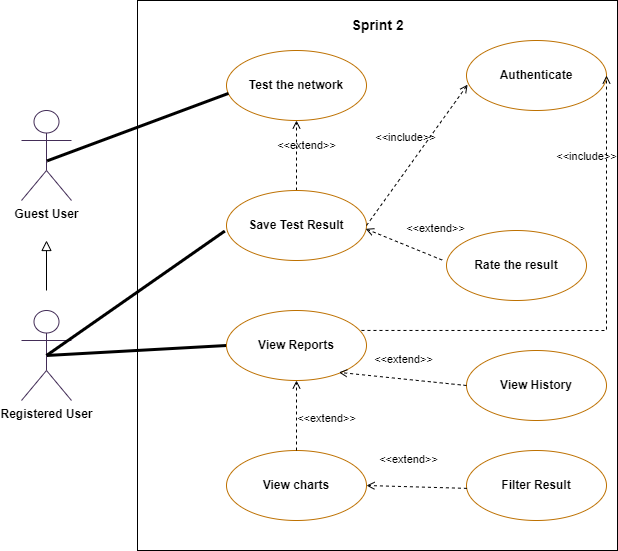
\includegraphics[width=0.98\textwidth]{images/sprint2/Sprint2UC.png}
     \caption{Sprint 2 Use Case Diagram}
    \label{fig:enter-label}
    
\end{figure}

\newpage
\section{User story n°1 : Network testing}
\textbf{\underline{Text description of the “Test the Network ” use case}}

\vspace{0.25cm}
We detail through this table the use case “Test the Network” :

\begin{table}[H]
    % \centering
    \renewcommand{\arraystretch}{1.5}
    
   \begin{tabular}{|p{0.25\textwidth}|p{0.68\textwidth}|}
   \hline
     
        \textbf{Use Case} & Test the network  \\   \hline
        
        \textbf{Actor(s) } & Guest user / Authenticated user   \\   \hline
        \textbf{Pre-condition} & 
           \begin{itemize}[left=0pt, label={\textbf{\Huge .}}]
            \item  The User request the testing page.
            \item  The device is connected to the internet.
        \end{itemize} 
        \\  \hline
        \textbf{Post-condition} & None \\   \hline


                \textbf{Principal scenario} &
                \begin{enumerate}[left=0pt]
                    \item The user launches the test.
                    \item The system retrieves some information about the user session (ip address,location,internet provider).
                    \item The system displays the retrieved data.
                    \item The system exchanges some chunks of data with the server .
                    \item After the receiving the last chunk of data, the system compute the metrics values.
                    \item The system displays the data and ask the user for saving the values in the database.
                    \item If the user confirms the values will sent to the database.
                
                    \end{enumerate}  \\   \hline

                     \textbf{Alternative\newline scenario} & 
        \begin{itemize}[left=0pt, label={\textbf{\Huge .}}]
            \item  If the device is not connected to the the internet a warning message appears.
        \end{itemize} \\   \hline
       
\end{tabular}

     \caption{Text Description Of The “Test the network” Use Case}
    \label{tab:my_label}
    
\end{table}

\newpage

\subsection{Sequence Diagram <<Test the network>> }



\begin{figure}[H]
   
    
    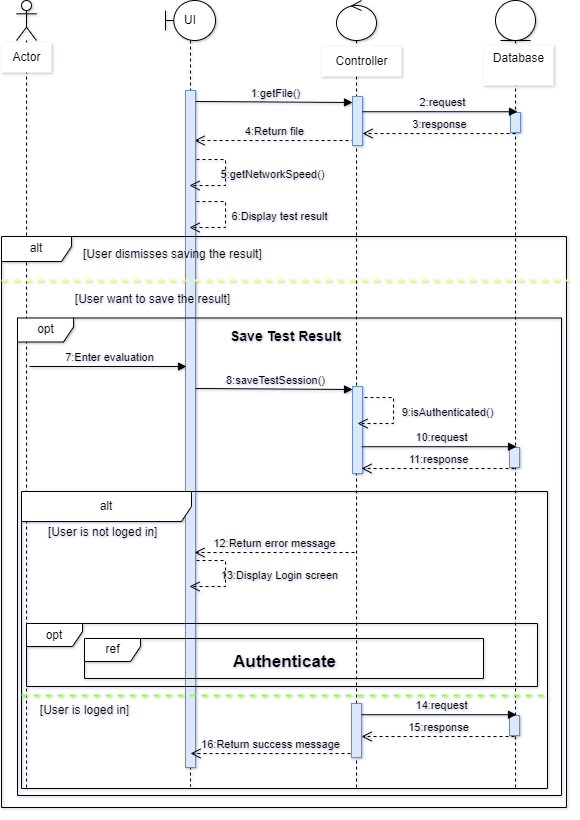
\includegraphics[width=0.98\textwidth]{images/sprint2/testNetworkSeq.png}
    \caption{“Test the network” Sequence Diagram}
    \label{fig:enter-label}
    
\end{figure}
\newpage
\subsection{Sprint 2 Class Diagram}
\begin{figure}[H]
   
    
    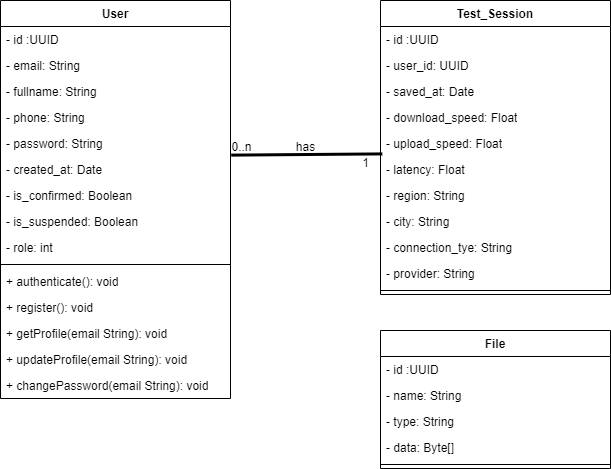
\includegraphics[width=0.98\textwidth]{images/sprint2/Sprint2ClassDiag.png}
    \caption{Sprint 2 Class Diagram}
    \label{fig:enter-label}
    
\end{figure}
\newpage
\subsection{Realization}
In the section we will explore the final user interfaces related to the user story n°1 : "Network Testing" in a sequential order :
\begin{figure}[H]
\begin{minipage}{0.32\textwidth}
    \centering
    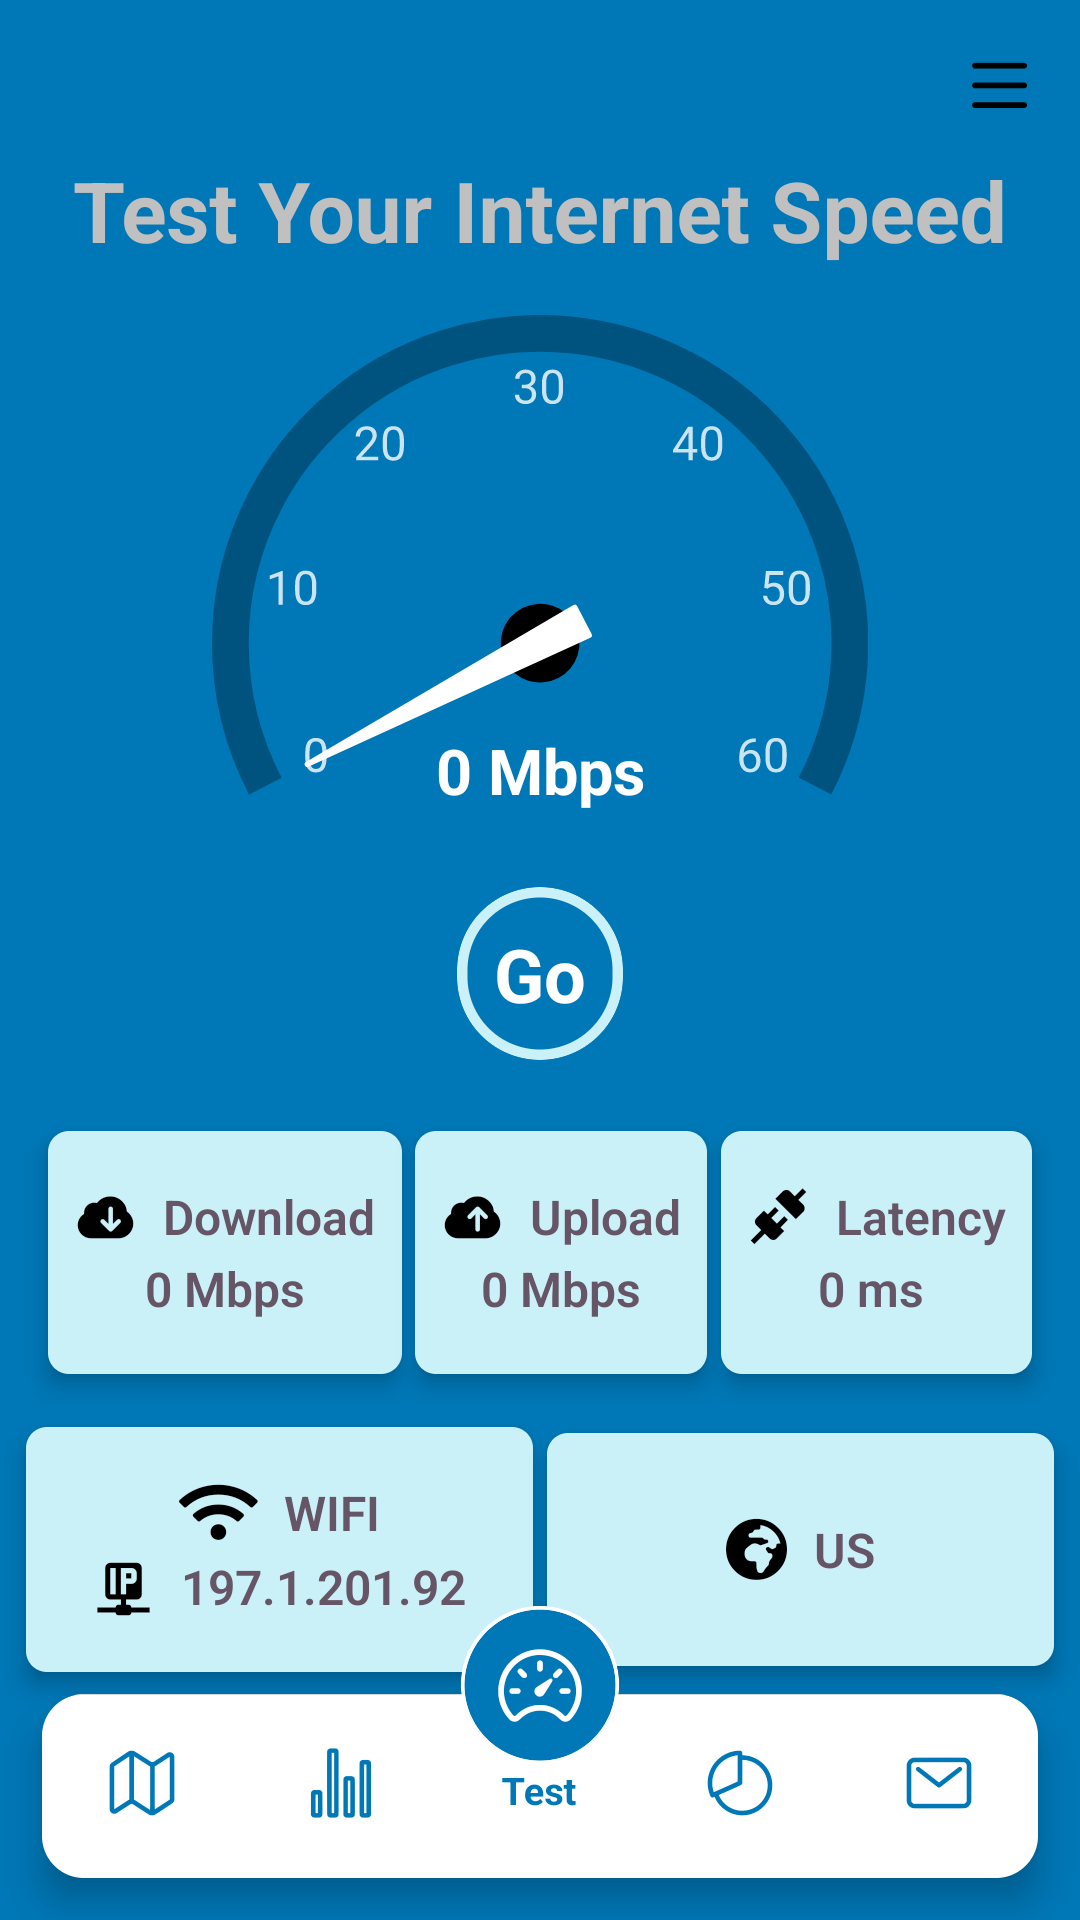
\includegraphics[width=\linewidth]{images/sprint2/testModuleInit.png}
    \label{fig:login-form-filled}
\end{minipage}\hfill
\begin{minipage}{0.3\textwidth}
    \centering
    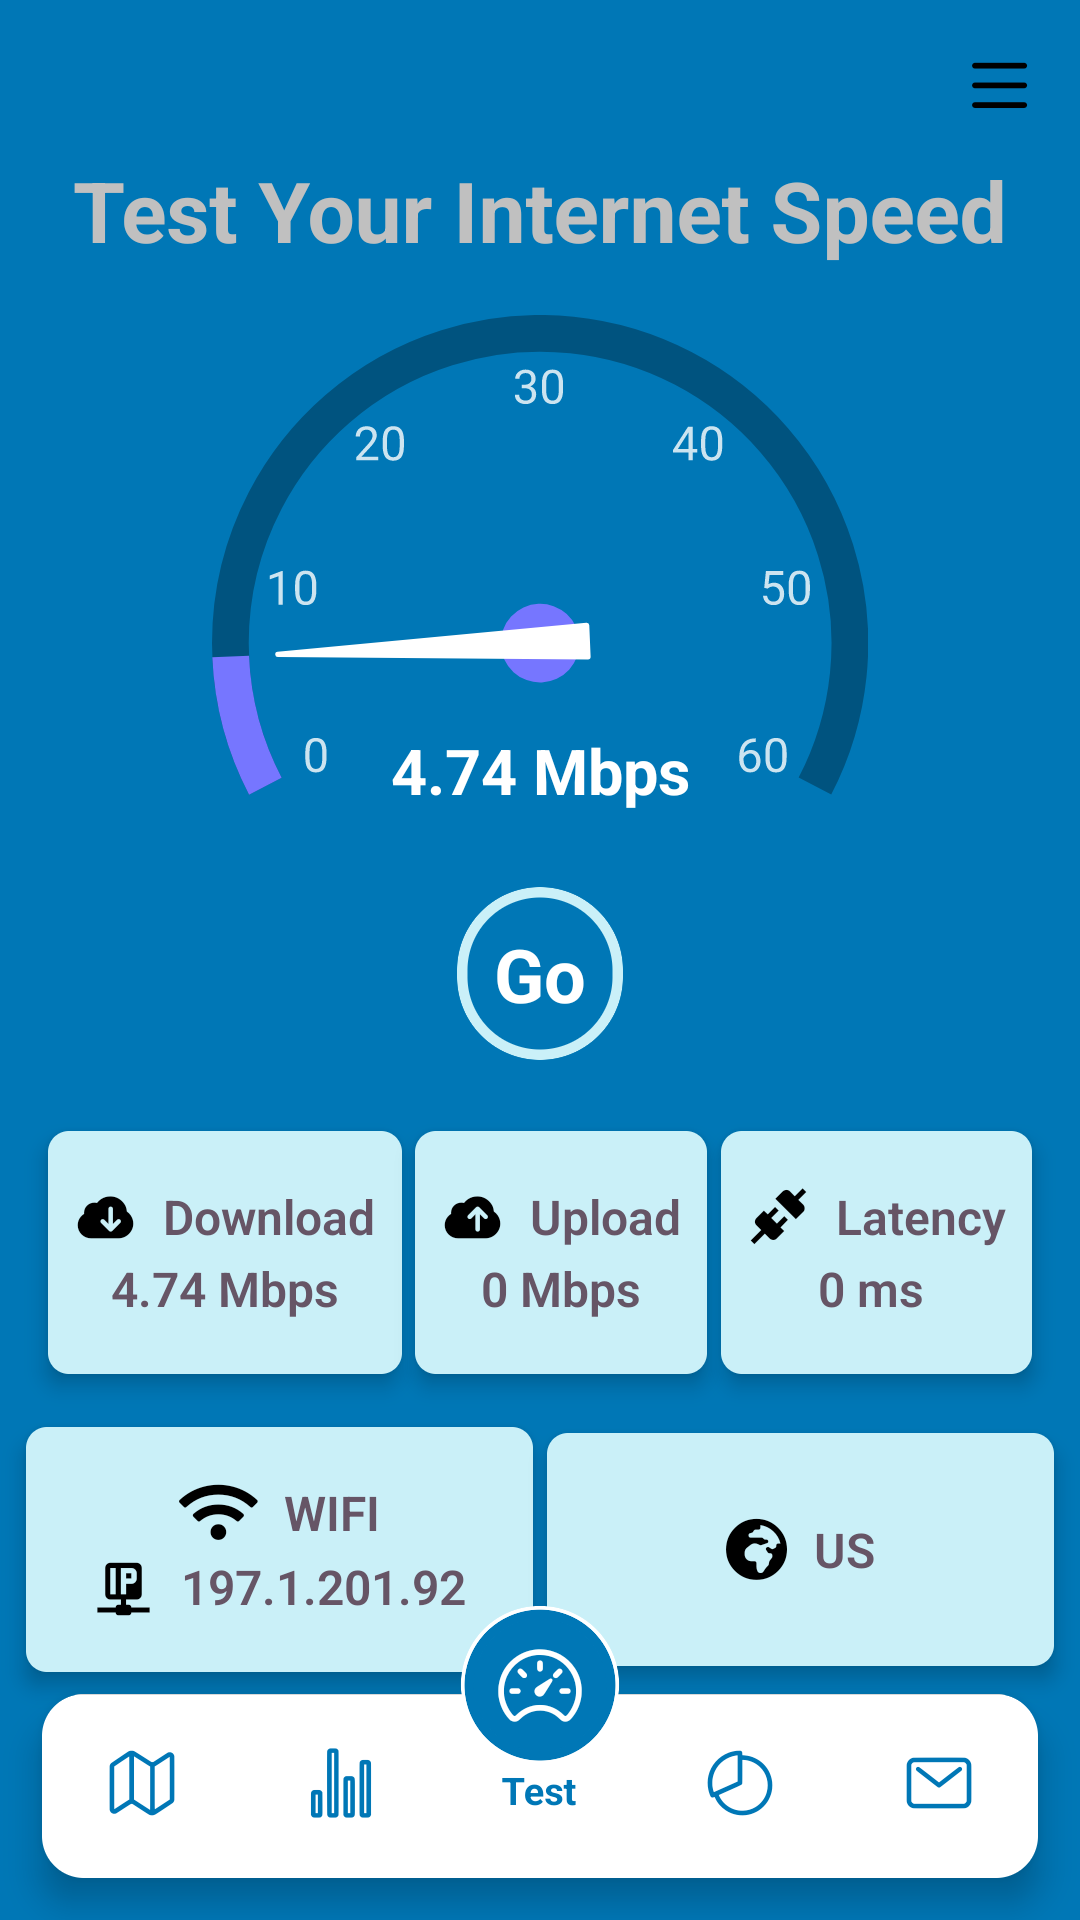
\includegraphics[width=\linewidth]{images/sprint2/testModuleActive.png}
    \label{fig:login-form}
\end{minipage}\hfill
\end{figure}
% \newpage
% After Finishing the test a modal like shown in the screen shot below appears
\begin{figure}[H]
\begin{center}
    \begin{minipage}{0.32\textwidth}
    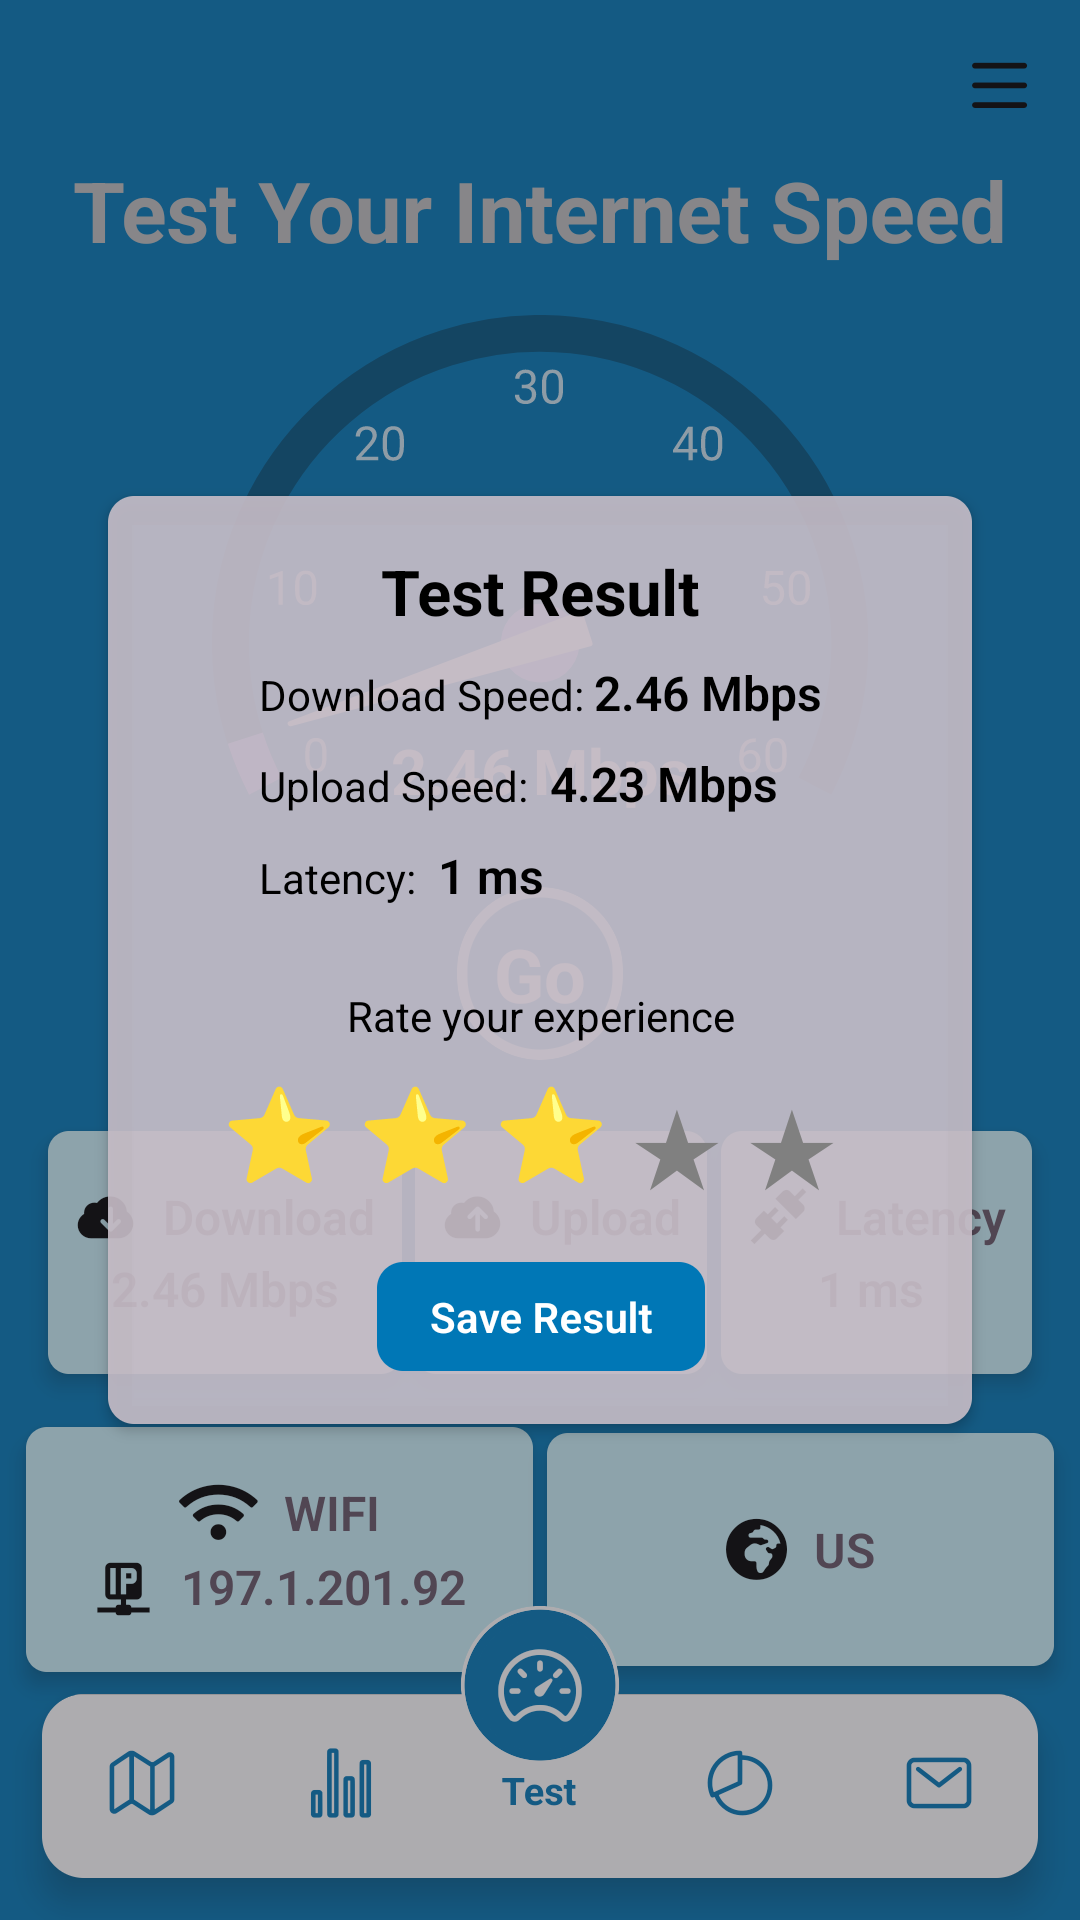
\includegraphics[width=\textwidth]{images/sprint2/testModuleFinish.png}
    \label{fig:enter-label}
    \end{minipage}\hfill
    \caption{Testing Screen}
\end{center}
\end{figure}


\newpage
\section{User story n°2 : Report generation}

\textbf{\underline{Text description of the “View Reports”use case:}}

\vspace{0.25cm}

We detail through this table the use case “View Reports” :

\begin{table}[H]
    % \centering
    \renewcommand{\arraystretch}{1.5}
    
   \begin{tabular}{|p{0.25\textwidth}|p{0.68\textwidth}|}
   \hline
     
        \textbf{Use Case} & View Reports  \\   \hline
        
        \textbf{Actor(s) } & Authenticated User  \\   \hline
        \textbf{Pre-condition} & The user requests the reports screen \\   \hline
        \textbf{Post-condition} & None  \\   \hline
                \textbf{Principal scenario} & 
                \begin{enumerate}
                    \item The user enters the reports screen.
                    \item The system retrieve the data related to the user .
                    \item The user interacts with the default charts.
                    \item The request an other chart.
                    \item The system extract the needed values and display the requested chart.
                \end{enumerate}  \\   \hline
        
        \textbf{Alternative\newline scenario} & 
        \begin{center}
            
        If user has not save any test yet a user friendly message appears.
        \end{center}
         \\   \hline
\end{tabular}
     \caption{Text Description Of The “View Reports” Use Case}
    \label{tab:my_label}
\end{table}


\newpage

\subsection{Sequence Diagram<<View Reports>> }
Below, we present the sequence diagrams for each use case mentioned above.

\begin{figure}[H]
   
    
    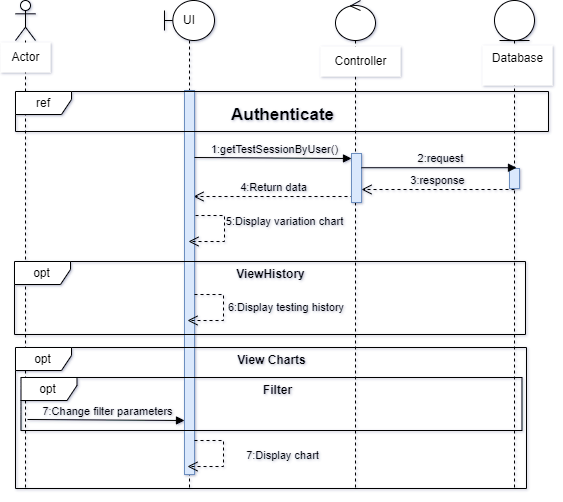
\includegraphics[width=0.98\textwidth]{images/sprint2/reportsSeq.png}
    \caption{News Feed - View News sequence diagram}
    \label{fig:enter-label}
    
\end{figure}
\newpage
\subsection{Realization}
In this section we will showcase the final outcome of the second user story of this sprint :
\begin{figure}[H]
\begin{minipage}{0.35\textwidth}
    \centering
    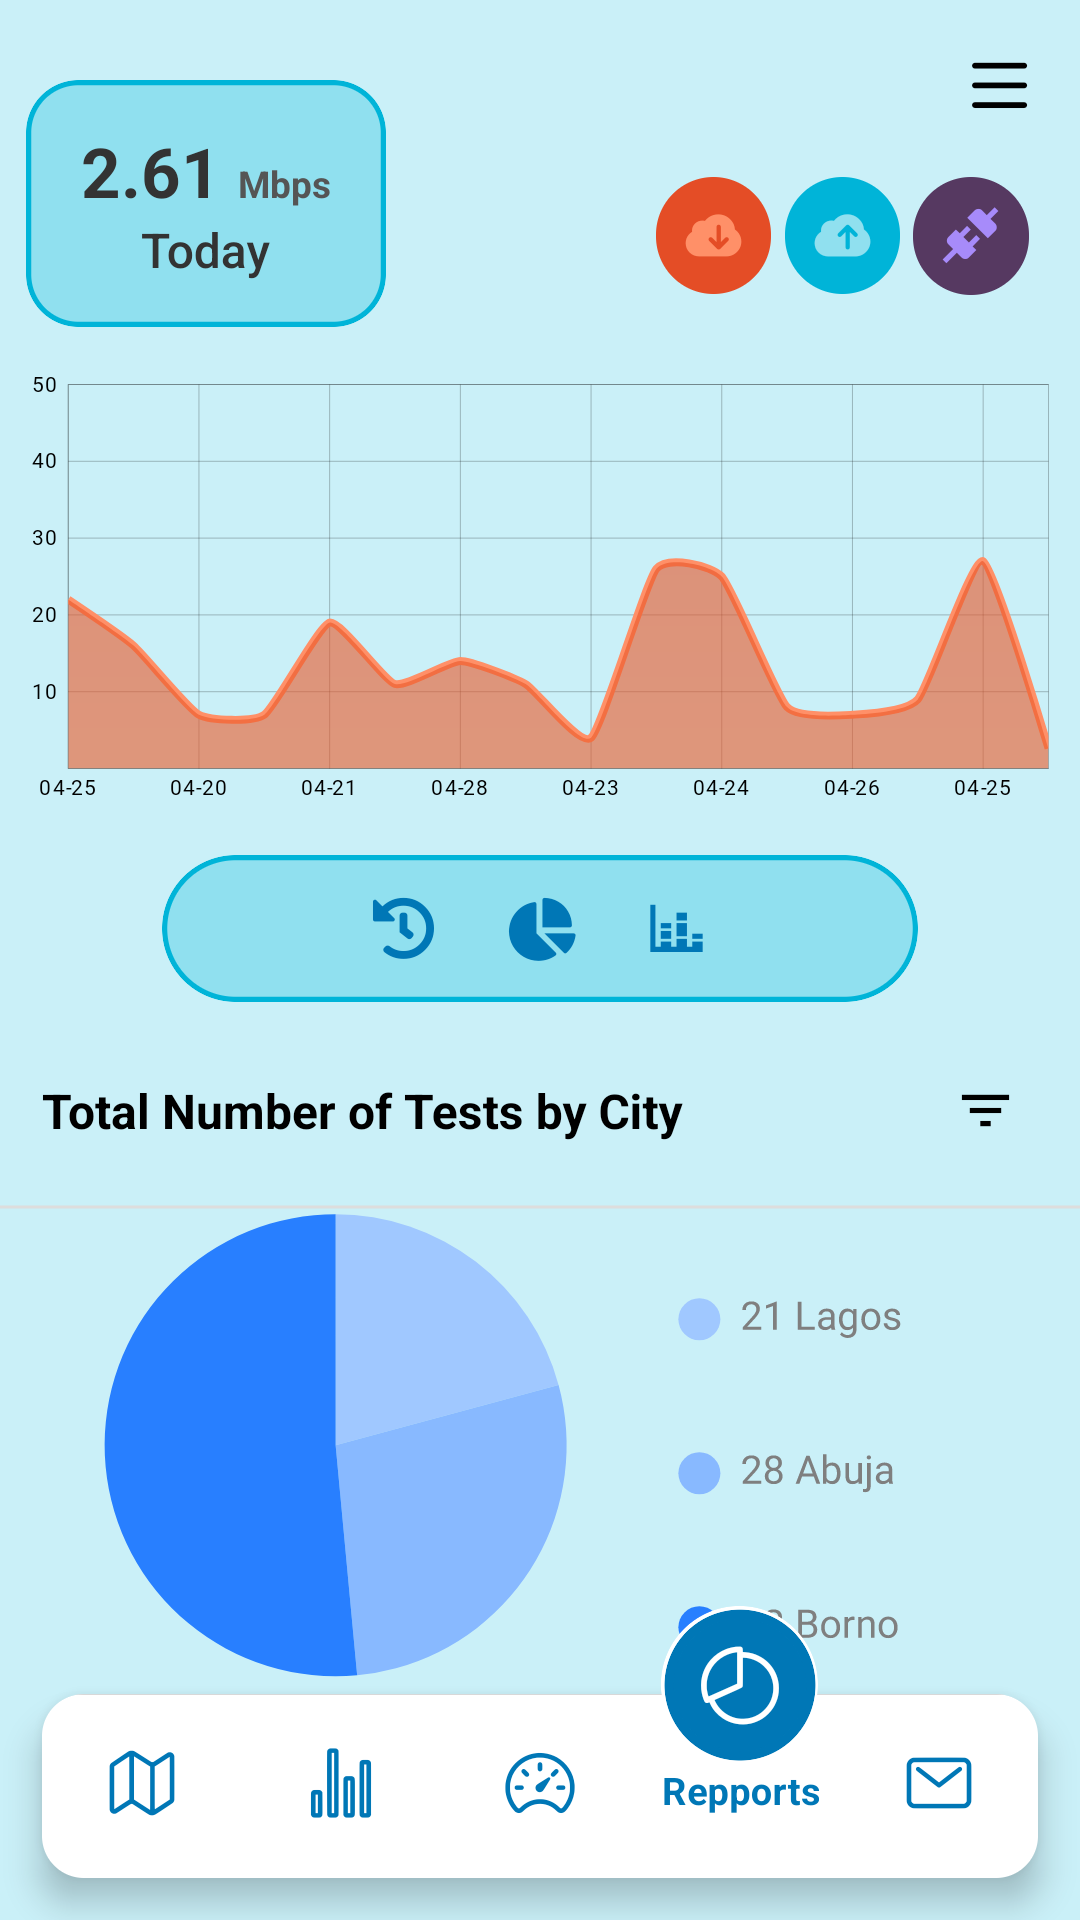
\includegraphics[width=\linewidth]{images/sprint2/ReportingModule (1).png}
    \label{fig:login-form-filled}
\end{minipage}\hfill
\begin{minipage}{0.35\textwidth}
    \centering
    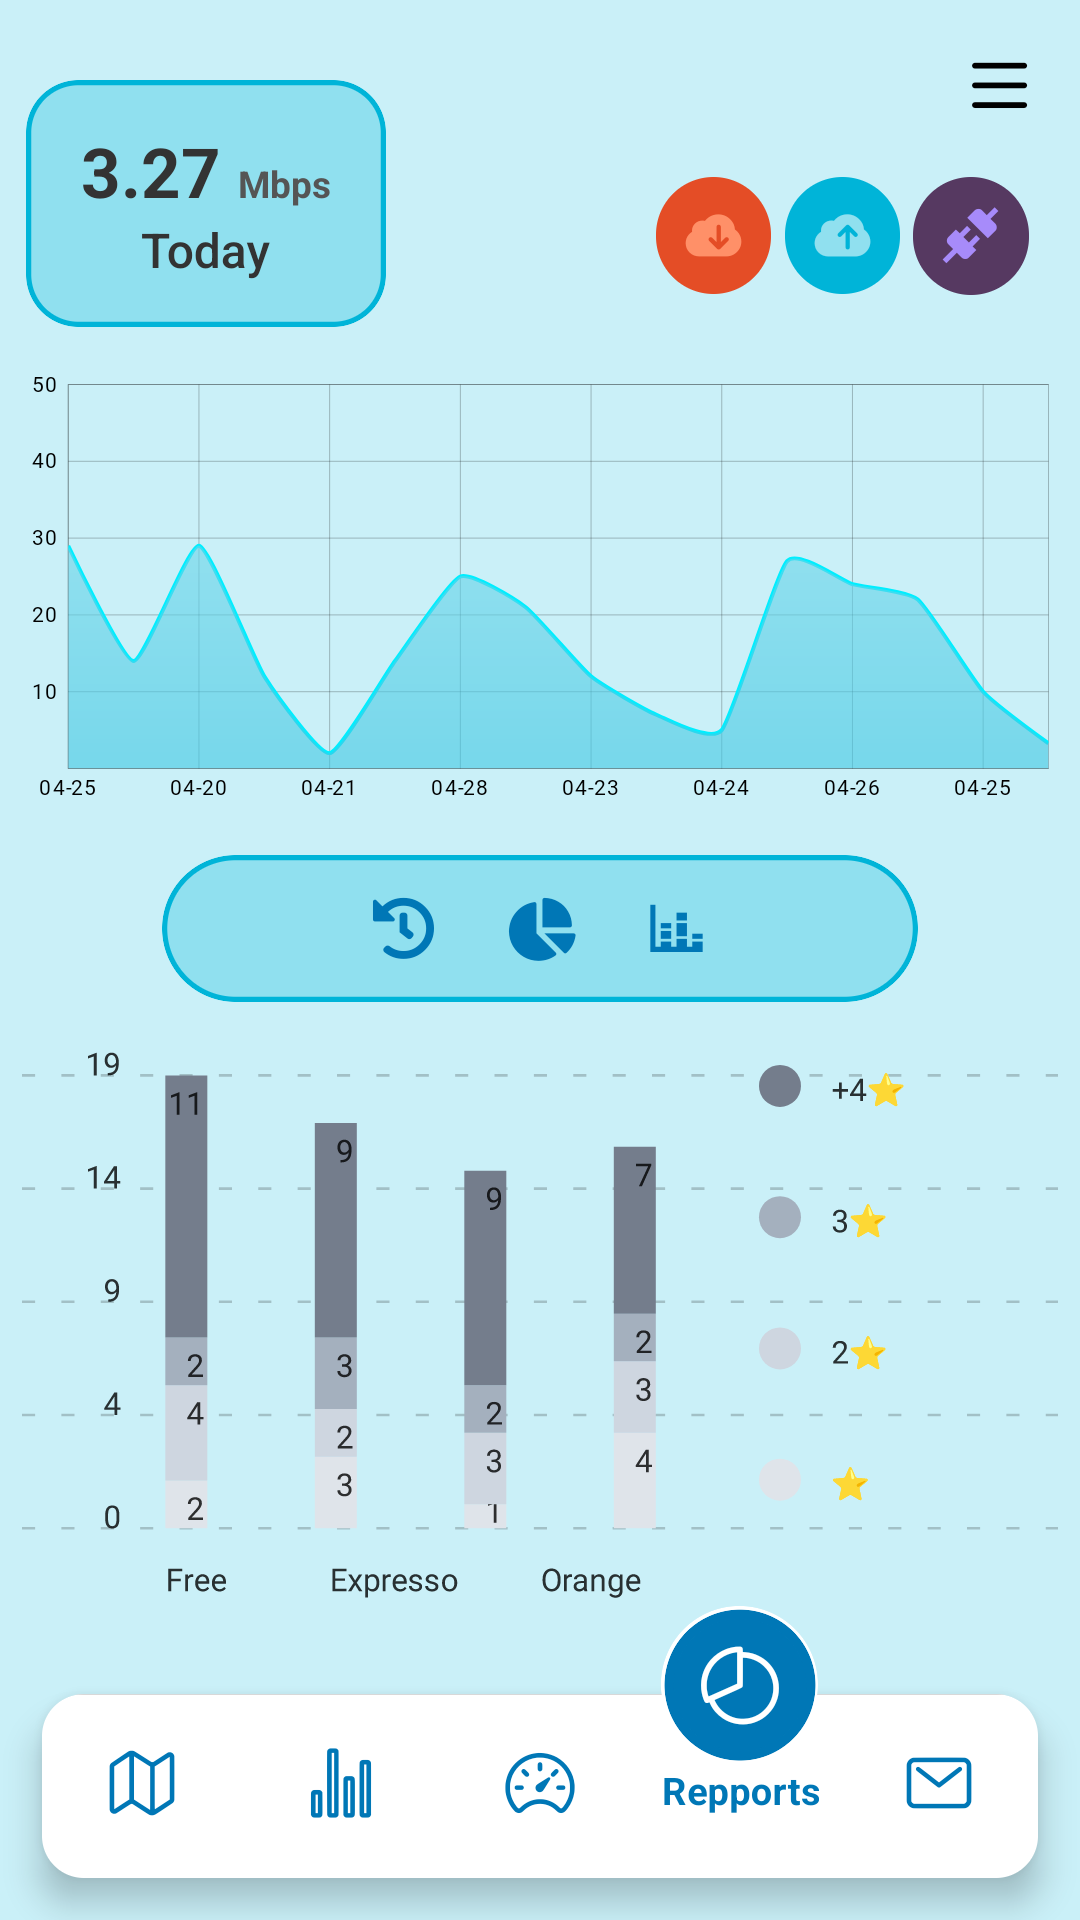
\includegraphics[width=\linewidth]{images/sprint2/ReportingModule (4).png}
    % \caption{Forget Password Sequence Diagram Part 1}
    \label{fig:login-form}
\end{minipage}\hfill
    % \caption{Reports Screen}
\end{figure}
\begin{figure}[H]
\begin{minipage}{0.35\textwidth}
    \centering
    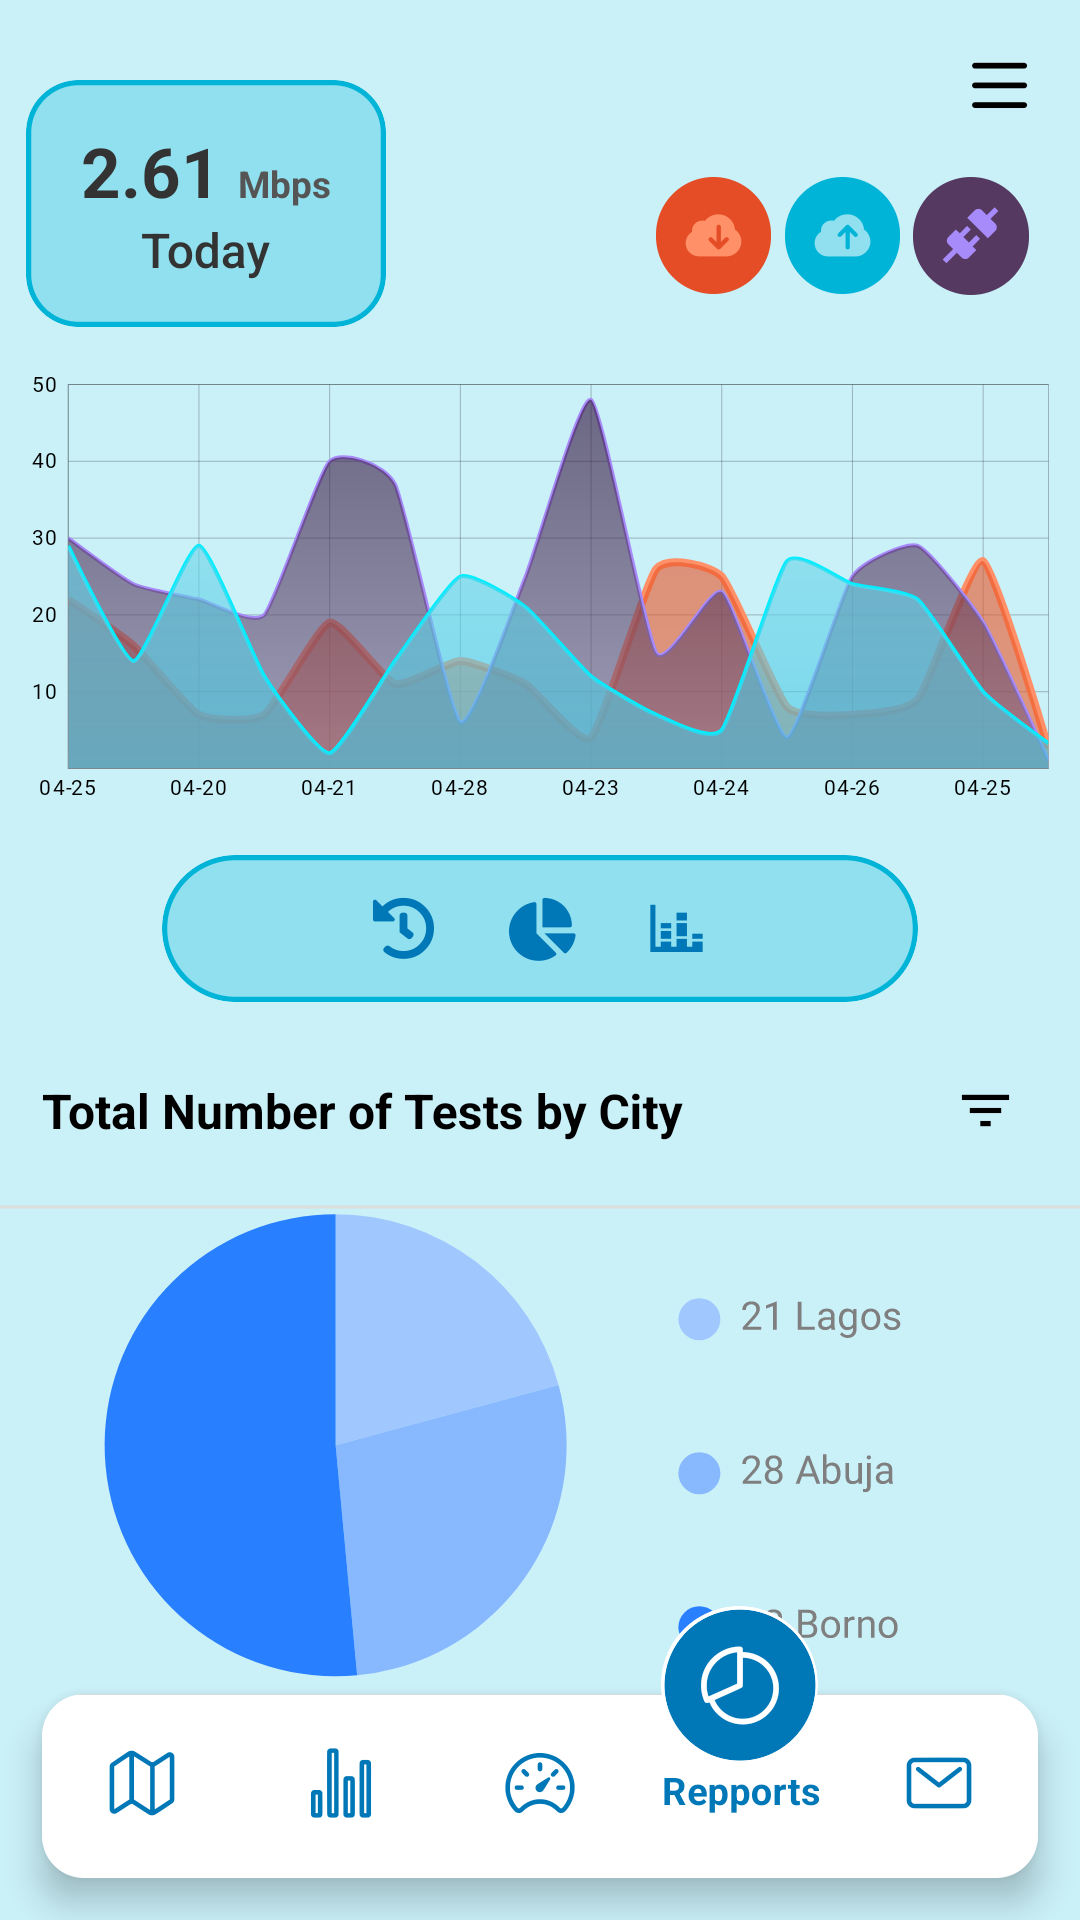
\includegraphics[width=\linewidth]{images/sprint2/ReportingModule (3).png}
    \label{fig:login-form-filled}
\end{minipage}\hfill
\begin{minipage}{0.35\textwidth}
    \centering
    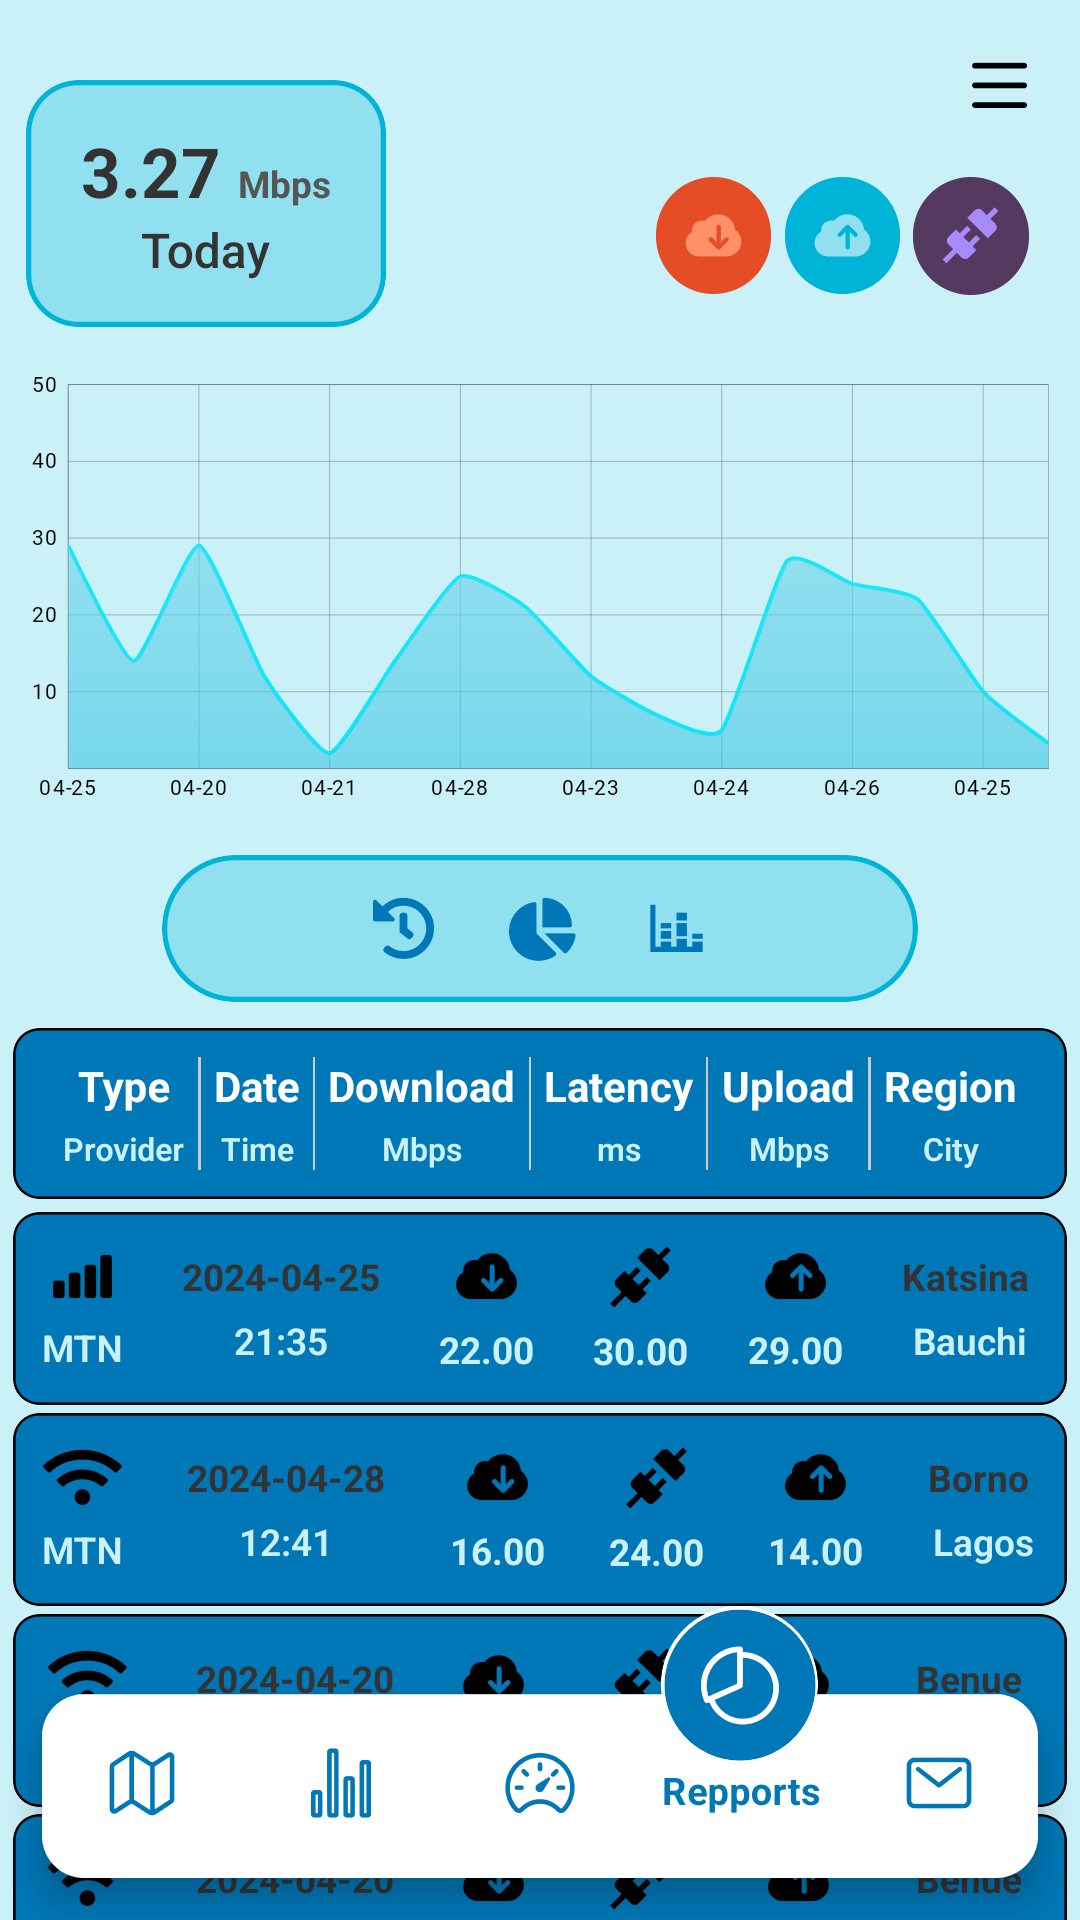
\includegraphics[width=\linewidth]{images/sprint2/ReportingModule (2).png}
    % \caption{Forget Password Sequence Diagram Part 1}
    \label{fig:login-form}
\end{minipage}\hfill
    \caption{Reports Screen}
\end{figure}


\section*{Conclusion}

Having concluded this chapter, we have effectively covered the analysis, modeling, and implementation of the second sprint, adding a critical component to our application. In the following chapter, we will face the challenging task of the 'Cartography' module.
